\section{AE21B045}

\section{{\color{blue}Introduction}}
A first-order reaction is one in which the rate of reaction is proportional to the concentration of the reactant. To put it another way, doubling the concentration doubles the reaction rate. A first-order reaction can have one or two reactants, as in the case of the decomposition reaction.
\section{{\color{blue}What is first order reaction?}}
A first-order reaction can be defined as a chemical reaction in which the reaction rate is linearly dependent on the concentration of only one reactant. In other words, a first-order reaction is a chemical reaction in which the rate varies based on the changes in the concentration of only one of the reactants. Thus, the order of these reactions is equal to 1.


\textbf{\textit{{\color{red}Examples of First-Order Reactions}}}
\\
\schemestart
\chemfig{SO_2Cl_2} 
\arrow{->}
{\chemfig{Cl_2}\+\chemfig{SO_2}}
\schemestop
\\
\schemestart
\chemfig{2N_2O_5}
\arrow{->}
{\chemfig{O_2}\+\chemfig{4NO_2}}
\schemestop
\section{{\color{blue}Differential Rate Law for a First-order Reaction}}
A differential rate law can be employed to describe a chemical reaction at a molecular level. The differential rate expression for a first-order reaction can be written as:
\\
\textbf{$Rate = -d[A]/dt = k[A]^1 = k[A]$}
\\
Where,
\begin{itemize}
\item ‘k’ is the rate constant of the first-order reaction, whose units are s-1.
\item ‘[A]’ denotes the concentration of the first-order reactant ‘A’.
\item d[A]/dt denotes the change in the concentration of the first-order reactant ‘A’ in the time interval ‘dt’
\end{itemize}
\section{{\color{blue}Integration Rate Law for a First-Order Reaction}}
Integrated rate expressions can be used to experimentally calculate the value of the rate constant of a reaction. To obtain the integral form of the rate expression for a first-order reaction, the differential rate law for the first-order reaction must be rearranged as follows.
\\
$$\frac{-d[A]}{dt} = k[A]$$
\\
$$\frac{d[A]}{[A]} = -kdt$$
\\
Integrating both sides of the equation, the following expression is obtained.
$$\int_{[A]}^{[A]_0} \frac{d[A]}{[A]} = -\int_{[t]}^{[t]_0}  kdt$$
\\
$$\int_{[A]}^{[A]_0}\frac{d[A]}{[A]} = - \int_{[t]}{[t]_0} kdt $$
\\
since
$$\int_{}^{}\frac{1}{x} = ln(x)$$

\\
the equation can be rewritten as follows:
\\
$$ln[A]-ln[A]_0 = -kt$$
\\
$$ln[A] = ln[A]_0-kt$$
\\
Raising each side of the equation to the exponent ‘e’ (since $$e^{ln(x)} = x$$), the equation is transformed as follows:
$$e^{ln[A]} = e^{ln[A]_0 - kt}$$
\\
Therefore,
$$[A] = [A]_0 e^{kt}$$
This expression is the integration from of the first-order rate law
\\

\section{{\color{blue}Graphical Representation of a First-Order Reaction}}

The concentration v/s time graph for a first-order reaction is provided below


\begin{figure}[b]
    
    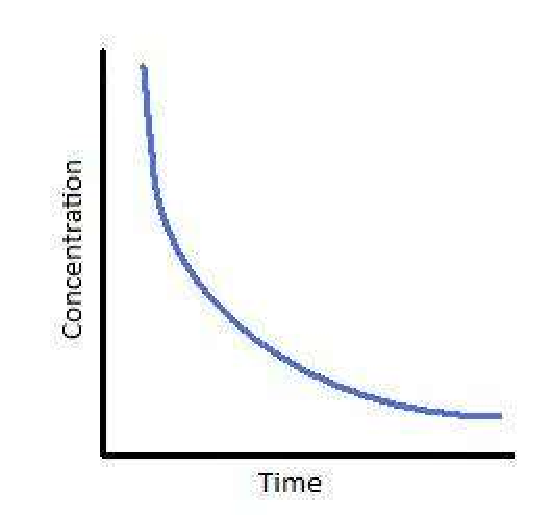
\includegraphics[scale=0.55]{jan-may-2022-latex/AE21B045/latexdash_compressed (1).pdf}
   \\
   For the first-order reactions, the equation $$ln[A]= -kt+ln[A]_0$$ is the similar to the straight line (y = mx+c) with slope -k. this line can be graphically plotted as follows
   \end{figure}
   

\begin{figure}[H]
   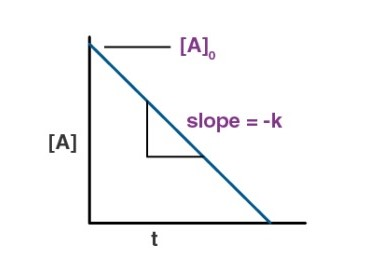
\includegraphics[scale=1]{jan-may-2022-latex/AE21B045/slopedited.jpeg}
   \caption{Thus, the graph for ln[A] v/s t for a first-order reaction is a straight line with slope -k.}
    \begin{tabular}{|l|l|l|l|l|l|l|}

\hline
Order & Reaction type & Differential rate law &Integrated RL& Half life & Units of k\\
\hline
    1 & R -> P & $$d[r]/dt = -k$$ & $$kt = [R]_0 - [R]$$ & [R]_0/2K& $$conc time^{-1}$$ \\
\hline
\end{tabular}
\end{figure}




